\documentclass[10pt]{article}
\usepackage[polish]{babel}
\usepackage[utf8]{inputenc}
\usepackage[T1]{fontenc}
\usepackage{amsmath}
\usepackage{amsfonts}
\usepackage{amssymb}
\usepackage[version=4]{mhchem}
\usepackage{stmaryrd}
\usepackage{graphicx}
\usepackage[export]{adjustbox}
\graphicspath{ {./images/} }

\begin{document}
\begin{enumerate}
  \item Znajdź wszystkie liczby całkowite \(k\), dla których \(\frac{k^{2}+1}{k+1}\) jest liczbą całkowitą.
  \item W trójkącie prostokątnym suma długości przyprostokątnych wynosi \(3 \sqrt{2}\), a przeciwprostokątna ma długość 4 . Oblicz pole tego trójkąta.
  \item W trójkącie ABC punkty D, E, F są środkami odpowiednio boków BC, CA i AB, a punkt G jest spodkiem wysokości opuszczonej z wierzchołka A. Udowodnij, że odcinki DE i FG mają jednakową długość.\\
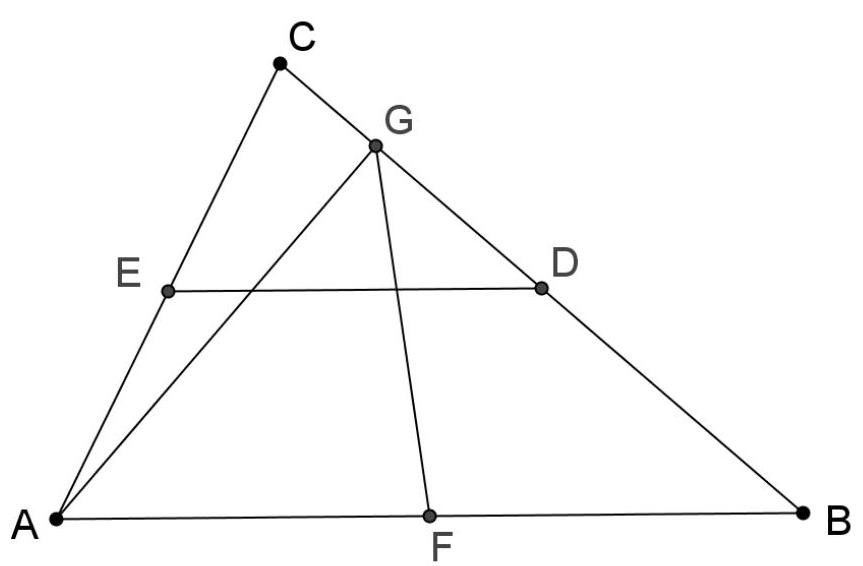
\includegraphics[max width=\textwidth, center]{2024_11_21_eb28af2003ece22058c4g-1}
\end{enumerate}

\end{document}